\documentclass[journal]{IEEEtran}
\usepackage[T1]{fontenc}
\usepackage{amsmath,amssymb}
\usepackage{graphicx}
\usepackage{booktabs}
\usepackage{multirow}
\usepackage{xcolor}
\usepackage[hidelinks]{hyperref}
\usepackage{cite}

% ---- facts the authors must confirm (red); see WRITING_NOTES.md ----
\newcommand{\RESULT}[1]{\textcolor{red}{[#1]}}
% auto-generated by me_attention.analysis -- do not edit

\newcommand{\BudgetT}{3}
\newcommand{\MaxEpochsE}{25}
\newcommand{\NBaselinesSpectral}{8}
\newcommand{\NBaselinesSpatial}{5}
\newcommand{\NBaselines}{13}
\newcommand{\NErrorRecords}{4}
\newcommand{\NRecords}{432}
\newcommand{\BestOursNamePepsinSpectral}{ex tokens v2}
\newcommand{\BestOursAccPepsinSpectral}{91.1}
\newcommand{\BestOursStdPepsinSpectral}{7.6}
\newcommand{\BestBaseNamePepsinSpectral}{LR}
\newcommand{\BestBaseAccPepsinSpectral}{90.3}
\newcommand{\GapPepsinSpectral}{$+0.8$}
\newcommand{\GapLoPepsinSpectral}{$-1.5$}
\newcommand{\GapHiPepsinSpectral}{$+3.1$}
\newcommand{\PWilcoxPepsinSpectral}{0.454}
\newcommand{\PNBPepsinSpectral}{0.823}
\newcommand{\PHolmPepsinSpectral}{0.454}
\newcommand{\NUnitsPepsinSpectral}{15}
\newcommand{\WinsPepsinSpectral}{9}
\newcommand{\TiesPepsinSpectral}{0}
\newcommand{\LossesPepsinSpectral}{6}
\newcommand{\BestOursNameLichensOneSpectral}{ex tokens v2}
\newcommand{\BestOursAccLichensOneSpectral}{98.8}
\newcommand{\BestOursStdLichensOneSpectral}{0.8}
\newcommand{\BestBaseNameLichensOneSpectral}{SpectralFormer}
\newcommand{\BestBaseAccLichensOneSpectral}{99.5}
\newcommand{\GapLichensOneSpectral}{$-0.6$}
\newcommand{\GapLoLichensOneSpectral}{$-1.3$}
\newcommand{\GapHiLichensOneSpectral}{$-0.1$}
\newcommand{\PWilcoxLichensOneSpectral}{0.250}
\newcommand{\PNBLichensOneSpectral}{0.306}
\newcommand{\PHolmLichensOneSpectral}{0.750}
\newcommand{\NUnitsLichensOneSpectral}{4}
\newcommand{\WinsLichensOneSpectral}{1}
\newcommand{\TiesLichensOneSpectral}{0}
\newcommand{\LossesLichensOneSpectral}{3}
\newcommand{\BestOursNameLichensTwoSpectral}{ex tokens v2}
\newcommand{\BestOursAccLichensTwoSpectral}{86.5}
\newcommand{\BestOursStdLichensTwoSpectral}{5.8}
\newcommand{\BestBaseNameLichensTwoSpectral}{RBF-SVM}
\newcommand{\BestBaseAccLichensTwoSpectral}{86.6}
\newcommand{\GapLichensTwoSpectral}{$-0.1$}
\newcommand{\GapLoLichensTwoSpectral}{$-1.0$}
\newcommand{\GapHiLichensTwoSpectral}{$+0.8$}
\newcommand{\PWilcoxLichensTwoSpectral}{1.000}
\newcommand{\PNBLichensTwoSpectral}{0.950}
\newcommand{\PHolmLichensTwoSpectral}{1.000}
\newcommand{\NUnitsLichensTwoSpectral}{10}
\newcommand{\WinsLichensTwoSpectral}{6}
\newcommand{\TiesLichensTwoSpectral}{0}
\newcommand{\LossesLichensTwoSpectral}{4}
\newcommand{\NDatasetsSpectral}{3}
\newcommand{\KFirstSpectral}{1}
\newcommand{\KSignificantSpectral}{0}
\newcommand{\GapMinSpectral}{$-0.6$}
\newcommand{\GapMaxSpectral}{$+0.8$}
\newcommand{\GapRangeSpectral}{$-0.6$ to $+0.8$}
\newcommand{\AvgRankCnnOneDSpectral}{9.08}
\newcommand{\AvgRankExTokensVTwoSpectral}{3.86}
\newcommand{\AvgRankHgbSpectral}{6.21}
\newcommand{\AvgRankHybridConvAttnSpectral}{8.70}
\newcommand{\AvgRankKnnSpectral}{9.09}
\newcommand{\AvgRankLrSpectral}{5.36}
\newcommand{\AvgRankMeasTokensSpectral}{7.04}
\newcommand{\AvgRankMlpSpectral}{6.01}
\newcommand{\AvgRankRbfsvmSpectral}{3.97}
\newcommand{\AvgRankRfSpectral}{7.35}
\newcommand{\AvgRankSmartattentionVZeroSpectral}{6.76}
\newcommand{\AvgRankSpectralformerSpectral}{4.57}
\newcommand{\CDNemenyiSpectral}{9.62}
\newcommand{\BestOursNamePepsinSpatial}{ME-Attn (spatial)}
\newcommand{\BestOursAccPepsinSpatial}{87.9}
\newcommand{\BestOursStdPepsinSpatial}{14.3}
\newcommand{\BestBaseNamePepsinSpatial}{Patch-mean RF}
\newcommand{\BestBaseAccPepsinSpatial}{86.4}
\newcommand{\GapPepsinSpatial}{$+1.4$}
\newcommand{\GapLoPepsinSpatial}{$-6.1$}
\newcommand{\GapHiPepsinSpatial}{$+7.7$}
\newcommand{\PWilcoxPepsinSpatial}{0.688}
\newcommand{\PNBPepsinSpatial}{0.862}
\newcommand{\PHolmPepsinSpatial}{0.688}
\newcommand{\NUnitsPepsinSpatial}{6}
\newcommand{\WinsPepsinSpatial}{4}
\newcommand{\TiesPepsinSpatial}{0}
\newcommand{\LossesPepsinSpatial}{2}
\newcommand{\BestOursNameLichensOneSpatial}{ME-Attn (spatial)}
\newcommand{\BestOursAccLichensOneSpatial}{99.1}
\newcommand{\BestOursStdLichensOneSpatial}{0.8}
\newcommand{\BestBaseNameLichensOneSpatial}{2D-CNN}
\newcommand{\BestBaseAccLichensOneSpatial}{99.6}
\newcommand{\GapLichensOneSpatial}{$-0.6$}
\newcommand{\GapLoLichensOneSpatial}{$-1.0$}
\newcommand{\GapHiLichensOneSpatial}{$-0.1$}
\newcommand{\PWilcoxLichensOneSpatial}{0.125}
\newcommand{\PNBLichensOneSpatial}{0.254}
\newcommand{\PHolmLichensOneSpatial}{0.125}
\newcommand{\NUnitsLichensOneSpatial}{4}
\newcommand{\WinsLichensOneSpatial}{0}
\newcommand{\TiesLichensOneSpatial}{0}
\newcommand{\LossesLichensOneSpatial}{4}
\newcommand{\BestOursNameLichensTwoSpatial}{ME-Attn (spatial)}
\newcommand{\BestOursAccLichensTwoSpatial}{85.6}
\newcommand{\BestOursStdLichensTwoSpatial}{1.9}
\newcommand{\BestBaseNameLichensTwoSpatial}{2D-CNN}
\newcommand{\BestBaseAccLichensTwoSpatial}{87.1}
\newcommand{\GapLichensTwoSpatial}{$-1.5$}
\newcommand{\GapLoLichensTwoSpatial}{$-3.6$}
\newcommand{\GapHiLichensTwoSpatial}{$-0.1$}
\newcommand{\PWilcoxLichensTwoSpatial}{0.125}
\newcommand{\PNBLichensTwoSpatial}{0.577}
\newcommand{\PHolmLichensTwoSpatial}{0.125}
\newcommand{\NUnitsLichensTwoSpatial}{4}
\newcommand{\WinsLichensTwoSpatial}{0}
\newcommand{\TiesLichensTwoSpatial}{0}
\newcommand{\LossesLichensTwoSpatial}{4}
\newcommand{\NDatasetsSpatial}{3}
\newcommand{\KFirstSpatial}{1}
\newcommand{\KSignificantSpatial}{0}
\newcommand{\GapMinSpatial}{$-1.5$}
\newcommand{\GapMaxSpatial}{$+1.4$}
\newcommand{\GapRangeSpatial}{$-1.5$ to $+1.4$}
\newcommand{\AvgRankCnnTwoDSpatial}{2.42}
\newcommand{\AvgRankPatchmeanLrSpatial}{4.06}
\newcommand{\AvgRankPatchmeanRfSpatial}{4.06}
\newcommand{\AvgRankSpatialAttnSpatial}{3.56}
\newcommand{\AvgRankSpectralformerPatchSpatial}{4.42}
\newcommand{\AvgRankSsfttSpatial}{2.50}
\newcommand{\CDNemenyiSpatial}{4.35}
 % auto-generated by me_attention.analysis
\newcommand{\lex}{\lambda^{\mathrm{ex}}}
\newcommand{\lem}{\lambda^{\mathrm{em}}}

\begin{document}

\title{Attention for Multi-Excitation Fluorescence Hyperspectral Pixel Classification: A Whole-Specimen Evaluation}

\author{First~Author,~Second~Author,~and~Third~Author%
\thanks{Manuscript in preparation. \RESULT{funding / acknowledgements}}}

\markboth{Draft}{Author \MakeLowercase{\textit{et al.}}: Attention for multi-excitation fluorescence HSI}

\maketitle

\begin{abstract}
Multi-excitation (ME) fluorescence hyperspectral imaging records an emission spectrum under several excitation wavelengths at each pixel, giving a sparse and irregular excitation--emission matrix (EEM). Random pixel splits can place neighbouring pixels from the same specimen in training and test sets and overstate generalisation. We therefore evaluate supervised ME-HSI classification with whole-specimen, class-covering folds. Hyperparameters are selected inside the outer training set, and all models use the same preprocessing options and the same number of candidate configurations. We compare four attention representations with 13 tuned baselines on Collagen Pepsin, Lichens~1 and Lichens~2. Tokenising one emission spectrum per excitation gives the highest mean among the proposed spectral models. It has the highest overall mean on Pepsin (\BestOursAccPepsinSpectral\,$\pm$\,\BestOursStdPepsinSpectral\% balanced accuracy), is 0.1 points below the RBF SVM on Lichens~2, and 0.6 points below SpectralFormer on Lichens~1. The corrected tests do not establish superiority over the strongest tuned baseline on any dataset. Measurement tokens, the reference prototype and the convolutional-stem hybrid have lower means on Pepsin and Lichens~2. The measurement-token attention ranking overlaps an unsupervised band-selection result more than expected by chance on Pepsin and Lichens~1, although the Lichens~1 rank correlation is weak. On the development set, random-pixel splits give about 98\% balanced accuracy for several models, compared with 87--88\% under whole-specimen evaluation. This 10--12 point protocol effect is larger than the differences among the leading models. The spatial experiments use annotation-derived specimen boundaries and are therefore treated as an oracle-boundary analysis rather than a deployment setting.
\end{abstract}

\begin{IEEEkeywords}
Hyperspectral imaging, fluorescence, excitation--emission matrix, attention, transformer, evaluation protocol, data leakage.
\end{IEEEkeywords}

\section{Introduction}
\IEEEPARstart{M}{ulti-excitation} (ME) fluorescence hyperspectral imaging (HSI) extends single-excitation fluorescence imaging by illuminating a specimen with several excitation wavelengths in turn and recording a full emission spectrum for each. The result is a four-dimensional array (two spatial axes, excitation, emission). Per pixel it is an excitation--emission matrix (EEM) of the kind long used in fluorescence spectroscopy, where the joint dependence on excitation and emission carries information that a single excitation does not~\cite{murphy2013parafac,bro1997parafac}. Endogenous fluorophores in tissue, such as collagen, NADH and elastin, differ in both their excitation and emission profiles~\cite{croce2014autofluorescence,monici2005autofluorescence}, and ME-HSI has been used to classify tissue states and to delineate lesions~\cite{gabrielyan2025access,hunanyan2025atrial,terpetrosyan2025configs}. Medical HSI more broadly is reviewed in~\cite{lu2014medical}.

In the setting of this paper, a tunable light source provides 6--8 excitation wavelengths between 310 and 430\,nm and a liquid-crystal tunable filter (LCTF) camera records emission between 420 and 750\,nm in 10\,nm steps. The resulting pixel is not a regular $E\times M$ matrix. Each excitation has its own emission window: the lower bound rises with the excitation wavelength (from 420\,nm to 470\,nm at 430\,nm excitation in the lichen data), the upper bound varies between 630 and 750\,nm, and for the shorter excitations of the collagen and lichen data a contiguous block of 70--90\,nm of bands is absent \RESULT{confirm reason for the removed block, e.g.\ excitation or second-order light}. In the lichen data the 415\,nm excitation is sampled on a grid offset by 5\,nm from the others. A classifier that treats the 150--210 measurements as an unordered, unlabelled feature vector discards the wavelength structure; one that assumes a regular grid must either interpolate or pad. Two natural questions follow. Does a model that knows the excitation and emission wavelength of each measurement classify better than one that does not? And does attention, which can relate measurements across excitations without a fixed layout, offer an advantage over convolutional, kernel and tree-based classifiers once all are tuned equally?

The second question cannot be answered reliably with the evaluation common in the HSI classification literature. Most benchmark protocols draw training and test pixels at random from the same image. Because neighbouring pixels are strongly correlated, such splits measure interpolation within a scene, not generalisation to new scenes or specimens, and the resulting accuracies are inflated~\cite{liang2017sampling,nalepa2019validating}. The same problem is known in other fields under the names spatial autocorrelation and data leakage~\cite{roberts2017cv,kapoor2023leakage}. For ME-HSI of biological specimens the relevant unit of generalisation is the specimen (a tissue sample, a lichen thallus), and the relevant error is the one made on a specimen that was never seen during training. In a preliminary analysis of our own earlier prototype we found two further sources of optimistic or unstable numbers: emission bands were aligned by index instead of by wavelength, and fold assignment did not guarantee that each test fold contained every class (Sec.~\ref{sec:motivation}). These issues are easy to miss in a single reported accuracy. They motivate a stricter whole-specimen evaluation protocol.

\textbf{Contributions.}
(i) A whole-specimen benchmark protocol and harness for ME-HSI with class-covering nested cross-validation, shared preprocessing, matched configuration counts, and paired statistical comparisons.
(ii) An attention family for irregular EEM data with measurement tokens, excitation tokens, a convolutional-stem hybrid, and a spatial extension. Relative wavelength bias is a searched option for the measurement-token model. Axial attention and gated tokens were implemented but were not part of the final sweep.
(iii) An evaluation against 13 tuned baselines. Excitation-level tokenisation has the strongest observed means within the proposed family, but no attention variant has a reliable advantage over the strongest tuned baseline on the three final datasets.
(iv) Evidence that the evaluation protocol has a larger effect than model choice on the development set: random-pixel splits raise balanced accuracy by 10--12 points relative to whole-specimen evaluation.
(v) A descriptive comparison showing above-chance set overlap between measurement-token attention rankings and an unsupervised wavelength-selection method~\cite{meloyan2026unsupervised}.

\section{Related Work}
\subsection{Deep learning for HSI classification}
Early deep models for HSI classification used 1D convolutions over the spectrum, 2D convolutions over spatial patches, and 3D convolutions over both~\cite{chen2016cnnhsi,hamida20183d}; a comparative review is given in~\cite{audebert2019review}. HybridSN stacks 3D and 2D convolutions to combine spectral and spatial features at moderate cost~\cite{roy2020hybridsn}; we implemented it but did not include it in the final comparison, where a 2D-CNN and SSFTT represent convolutional spectral--spatial models. Transformers~\cite{vaswani2017attention,dosovitskiy2021vit} entered the field through SpectralFormer, which embeds groups of neighbouring bands as tokens and adds cross-layer feature fusion~\cite{hong2022spectralformer}, and SSFTT, which builds tokens from 3D--2D convolutional features with a Gaussian-weighted tokenizer~\cite{sun2022ssftt}. Foundation models such as SpectralGPT are pre-trained on large collections of spectral remote sensing images~\cite{hong2024spectralgpt}. These models assume that the spectral axis is a regular, ordered sequence of broad-band or narrow-band channels, and positional information is learned or implied by index. ME fluorescence data do not fit this assumption: the measurements are indexed by two wavelengths, the grid is irregular, and neighbouring indices need not be neighbouring wavelengths. We therefore include SpectralFormer and SSFTT as baselines adapted to our feature layout, and design the attention family around wavelength-valued, not index-valued, positions.

\subsection{Fluorescence EEM analysis}
EEMs are classically analysed with multi-way decompositions such as PARAFAC, which factor a stack of EEMs into excitation and emission loadings under a trilinear model~\cite{bro1997parafac,murphy2013parafac}. These methods are unsupervised, assume a regular grid after correction of scatter and missing regions, and operate on samples (or on pixels as samples) in aggregate. Our setting is supervised and per-pixel, and the model must tolerate missing and irregular cells.

\subsection{Evaluation leakage in HSI classification}
Liang \emph{et al.} showed that random sampling of training pixels in scenes with spatially extended classes produces over-optimistic accuracy for spectral--spatial methods, because training and test patches overlap, and argued for spatially disjoint sampling~\cite{liang2017sampling}. Nalepa \emph{et al.} reached a similar conclusion for HSI segmentation and proposed leakage-free validation~\cite{nalepa2019validating}. General treatments of cross-validation for structured data are found in~\cite{roberts2017cv}, and a survey of leakage in ML-based science in~\cite{kapoor2023leakage}. Our protocol follows this line and enforces three additional constraints: folds hold out complete specimens, every test fold contains every class, and model selection uses held-out specimens inside the training set, in the spirit of nested cross-validation~\cite{cawley2010overfitting}.

\subsection{Generalisation across specimens and domains}
Specimen-to-specimen variation (preparation, thickness, exposure, ageing) is a form of domain shift. Domain generalisation methods address it with invariance objectives, data augmentation and regularisation~\cite{zhou2022dgsurvey,wang2022dgsurvey}, and a careful comparison found that tuned empirical risk minimisation is a strong baseline when model selection and budget are controlled~\cite{gulrajani2021domainbed}. We adopt the second lesson as a design constraint: every model, ours and the baselines, gets the same tuning budget and model-selection rule.

\section{Data}
\subsection{Acquisition}
Specimens were imaged with a tunable-source ME fluorescence system. For each excitation wavelength, an emission cube was recorded with an LCTF camera at 10\,nm steps from 420\,nm up to 720\,nm (collagen, Lichens~1) or 750\,nm (Lichens~2). Exposure time and lamp power were recorded per excitation and used to put measurements on a common radiometric scale before analysis \RESULT{confirm radiometric correction applied to each dataset}. Excitation wavelengths are 310, 325, 340, 365, 385 and 400\,nm for the collagen data and additionally 415 and 430\,nm for the lichen data. Each excitation therefore keeps its own set of emission bands (windows of 24--31 bands per excitation in the collagen data and 22--30 in the lichen data), and the cube is ragged. In both lichen datasets the 415\,nm excitation is sampled at 455, 465, \dots\,nm, i.e.\ in 10\,nm steps on a grid offset by 5\,nm from the other excitations, which gives union emission grids of $M=55$ (Lichens~1) and $M=63$ (Lichens~2) distinct wavelengths for 8 excitations. Spatial size is $256\times348$ pixels for the collagen data and Lichens~2, and $1040\times925$ for Lichens~1.

\subsection{Datasets and specimens}
Class labels are given by a region mask drawn on the image. A \emph{specimen} is an 8-connected component of one class in the mask; components with fewer than 100 pixels are discarded (none for Collagen Pepsin and Lichens~1, one component of 18 pixels for Lichens~2, and one of 11 pixels for the development set). For Collagen Pepsin and Lichens~1, these components correspond to physically separate samples. Lichens~2 is a different processed representation of the same underlying lichen material as Lichens~1, rather than an independent biological cohort. Its ``specimens'' are spatially disjoint annotated regions and may not be biologically independent (Sec.~\ref{sec:limits}). Table~\ref{tab:data} summarises the data.

\begin{table*}[!t]
\centering
\caption{Datasets. $S_c$: specimens or annotated regions per class; $E$: excitations; $M$: distinct emission wavelengths in the union grid; $F$: valid (excitation, emission) measurements per pixel. Collagen Acetic Acid is used only for development analyses and is not part of the final benchmark tables. Lichens~1 and Lichens~2 are not independent biological cohorts.}
\label{tab:data}
\small
\begin{tabular}{lcccrcccl}
\toprule
Dataset & Classes & $S_c$ & Pixels & Excitations (nm) & $E$ & $M$ & $F$ & Emission (nm) \\
\midrule
Collagen Pepsin & 3 & 3/3/3 & 39\,970 & 310--400 & 6 & 31 & 158 & 420--720 \\
Lichens 1 & 4 & 4/4/4/4 & 191\,046 & 310--430 & 8 & 55 & 192 & 420--720 \\
Lichens 2 & 5 & 4/10/7/5/2 & 22\,562 & 310--430 & 8 & 63 & 210 & 420--750 \\
\midrule
Collagen Acetic (dev.) & 3 & 3/3/3 & 46\,670 & 310--400 & 6 & 31 & 149 & 420--720 \\
\bottomrule
\end{tabular}
\end{table*}

The two collagen datasets have the same number of excitations, union-grid size and nominal emission range, but different $F$ because the retained valid excitation--emission cells differ after preprocessing.

\subsection{Irregular emission grids}
Models must not assume a regular $E\times M$ grid. All loaders align measurements by their wavelength in nanometres and refuse to fall back to index alignment when a cube lacks a wavelength vector. Features are stored as a flat list of valid measurements sorted by (excitation, emission), with the arrays $\lex_i$, $\lem_i$ and the grid position $(e_i,m_i)$ of each feature. Models that need a grid scatter the features onto $E\times M$ and carry a validity mask.

\section{Method}
\subsection{Problem formulation}
Let a pixel be a set of $F$ valid measurements $\{(\lex_i,\lem_i,x_i)\}_{i=1}^{F}$ with $x_i\ge 0$ the recorded intensity. In the spectral track the classifier $f:\{(\lex_i,\lem_i,x_i)\}\to \Delta^{C-1}$ maps one pixel to class probabilities. The spatial track receives a $P\times P$ patch centred on the pixel. Pixels outside the centre pixel's annotated specimen or region are set to zero. This prevents context from crossing annotated component boundaries, but the boundary mask is derived from the annotation and is therefore oracle information at test time. Both tracks hold out complete outer-test components during training.

\subsection{Measurement-set representation}
Intensities are preprocessed with a shared, non-trainable preprocessing transform (Sec.~\ref{sec:preproc}); the model sees standardised features $\tilde x_i$. Each measurement is a token, so the number of tokens is the number of valid cells and no padding or interpolation is needed. Wavelengths enter as continuous quantities, not indices.

\subsection{Attention family}
\begin{figure*}[!t]
\centering
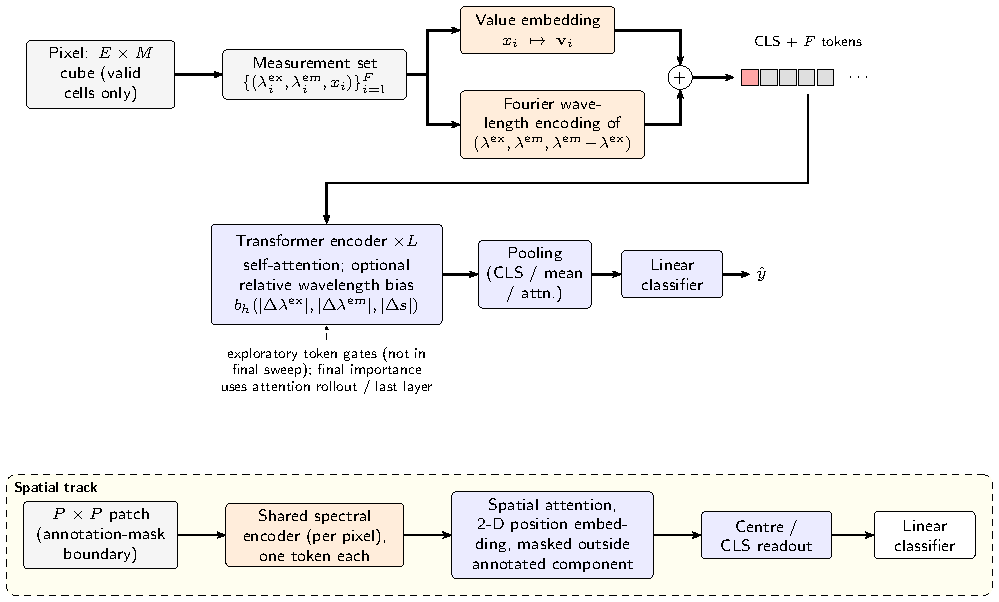
\includegraphics[width=0.92\textwidth]{figures/fig_arch.pdf}
\caption{Measurement-token attention model (top) and its spatial extension (bottom). A pixel is a set of (excitation, emission, intensity) measurements. Each token combines a value embedding with a Fourier encoding of $(\lex,\lem,\lem-\lex)$. Relative wavelength bias is an optional searched component; token gates were implemented only as an exploratory variant. In the spatial track a shared spectral encoder maps every patch pixel to a token and a second attention stage reads out the centre pixel. The spatial mask uses annotation-derived component boundaries.}
\label{fig:arch}
\end{figure*}
\begin{figure*}[!t]
\centering
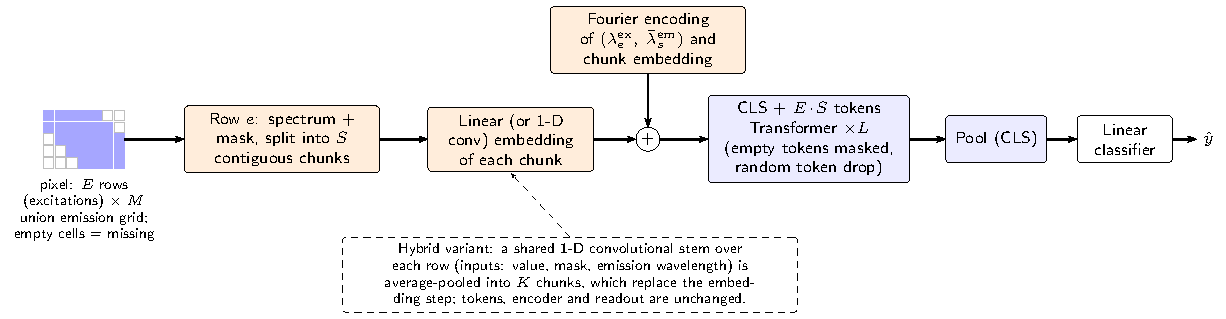
\includegraphics[width=0.92\textwidth]{figures/fig_extokens.pdf}
\caption{Excitation-token model. Each excitation's emission spectrum on the union grid (with a validity mask) is split into $S$ chunks, embedded, and combined with a Fourier encoding of the excitation and chunk-centre emission wavelengths; a transformer over the $E\cdot S$ tokens and a CLS readout give the prediction. The hybrid variant (dashed) replaces the embedding by a shared 1-D convolutional stem and pooling into $K$ chunks.}
\label{fig:extokens}
\end{figure*}

Fig.~\ref{fig:arch} shows the measurement-token model, one member of the family, and Fig.~\ref{fig:extokens} shows the excitation-token model and the hybrid variant. The components below are options; their configuration is chosen by inner validation (Sec.~\ref{sec:protocol}) within the frozen search spaces. Four spectral members were evaluated: the corrected prototype, measurement tokens, excitation tokens and the conv-stem hybrid.

\subsubsection{Measurement tokens with continuous wavelength encoding}
Token $i$ is $\mathbf{t}_i=\phi(\tilde x_i)+\psi(\lex_i,\lem_i,s_i)$ with Stokes shift $s_i=\lem_i-\lex_i$. The value embedding $\phi$ is a learned scale-and-shift vector or a small MLP. The wavelength encoding $\psi$ rescales the three quantities to $[0,1]$ and applies Fourier features~\cite{tancik2020fourier}: for $u\in[0,1]$, $\gamma(u)=[u,\sin(2\pi k u),\cos(2\pi k u)]_{k=1}^{K}$, followed by a linear map to the model width. A learned per-feature embedding is available as an alternative. A classification token is prepended, or tokens are pooled by a learned-query attention (searched: Fourier or Fourier-plus-learned encoding, with or without relative bias, CLS or attention pooling). With 150--210 tokens this is the most expensive member. The encoder is a pre-norm transformer~\cite{vaswani2017attention} with stochastic depth and optional random dropping of measurement tokens during training.

\subsubsection{Relative wavelength bias}
Following relative position representations~\cite{shaw2018relpos} and learned relative biases~\cite{raffel2020t5}, attention logits can receive an additive per-head bias $b_h=\mathrm{MLP}_h(|\Delta\lex|,|\Delta\lem|,|\Delta s|)$, with distances normalised by the corresponding wavelength range. The last layer is zero-initialised, so training starts from plain attention. Relative bias is included as a measurement-token search-space option. We did not run a dedicated ablation that isolates its effect.

\subsubsection{Axial attention on the EEM (implemented, not evaluated)}
Tokens are placed on the $E\times M$ grid and blocks alternate attention along emission (within one excitation) and along excitation (at one emission wavelength), with key-padding masks for missing cells. This restricts attention to the two axes along which EEMs are physically structured and reduces cost from $O(F^2)$ to $O(E M^2+M E^2)$. It was implemented and gave a competitive result on the development set (85.3\%) but is not part of the final sweep, for cost and redundancy with the excitation-token model.

\subsubsection{Excitation tokens}\label{sec:extok}
The excitation-token model (\texttt{ex\_tokens\_v2}, Fig.~\ref{fig:extokens}) forms one token per excitation from that excitation's emission spectrum. The $F$ features are scattered onto the $E\times M$ union grid, missing cells are set to zero, and a binary validity mask is a second channel. The emission axis is zero-padded to a multiple of $2S$ and split into $S$ contiguous chunks ($S=1$ by default, i.e.\ one token per excitation, or $S=2$ sub-tokens). Each chunk, with its mask, is embedded by a single linear layer (default) or by a small 1-D convolution (two $k{=}5$ layers, 16 channels, input channels value, mask and normalised emission wavelength) followed by a linear layer. The token is the sum of this embedding, a Fourier encoding of the pair (excitation wavelength, chunk-centre emission wavelength) with $K{=}8$ frequencies, and a learned chunk embedding. Tokens whose chunk contains no valid cell are masked as keys, and during training further tokens are dropped at random (probability 0.1). A classification token is prepended and a pre-norm transformer encoder (default width 64, depth 3, 4 heads, MLP ratio 2) acts on the $E$ (or $ES$) tokens; the classification token feeds a linear classifier (mean pooling over valid tokens is available). The searched options are width $\{32,64\}$, depth $\{2,3\}$, sub-tokens $\{1,2\}$ and dropout $\{0.1,0.3\}$; the linear embedding and CLS pooling are fixed. Cross-excitation interactions are explicit. With $E\in\{6,8\}$ and $S\in\{1,2\}$, the model uses 6--16 excitation/chunk tokens before the CLS token. The default $S=1$ configuration uses 6--8 such tokens.

\subsubsection{Hybrid convolutional-stem attention}
\texttt{hybrid\_conv\_attn} replaces the chunk embedding by a learned local feature extractor. A stem of two 1-D convolutions ($k{=}5$, 24 channels, GELU; input channels value, mask and normalised emission wavelength) is shared across excitations and applied along the emission axis of each excitation row. Its output is average-pooled into $K$ contiguous chunks of the union grid, projected to the model width, and given the same Fourier encoding of (excitation, chunk-centre emission) as above, giving $E\cdot K$ (excitation, chunk) tokens. A CLS token, a transformer encoder (default width 64, depth 2, 4 heads) and a linear classifier follow, with the same token masking and token dropout as the excitation-token model. The searched options are width $\{32,64\}$, depth $\{1,2,3\}$, chunks $K\in\{4,6,8\}$ and dropout $\{0.1,0.3\}$.

\subsubsection{Gated tokens (implemented, not in the frozen search space)}
A learned gate $g_i=\sigma(\theta_i)$ per measurement scales the token and is added as $\log g_i$ to the attention logits of that key. An $L_1$ penalty on the mean gate encourages sparsity. Gates were not part of the frozen final sweep and are not used in the importance analysis below. That analysis uses attention rollout~\cite{abnar2020flow} and last-layer attention, both treated as descriptive rather than causal~\cite{jain2019notexpl}.

\subsubsection{Reference prototype}
The prototype (\texttt{smartattention\_v0}) is a SpectralFormer-style model in which tokens are emission positions carrying the intensities of all excitations and their two spectral neighbours, with cross-layer feature fusion. It is evaluated on the aligned wavelength grid (after the grid-alignment correction of Sec.~\ref{sec:motivation}) and is included as a model, not as a baseline, to show the effect of the more general tokenisations.

\subsection{Spatial extension}
For the spatial track a shared spectral encoder (an excitation-token encoder or an MLP, chosen by the search) maps each valid pixel in the $P\times P$ patch to one token. A 2-D learned position embedding is added, pixels outside the centre pixel's annotated component are masked as keys, and a second transformer attends over the pixel tokens. The prediction is read from a classification token or from the centre token, optionally concatenated with the centre pixel's own spectral embedding. Patch size is tuned in $\{5,7\}$. Because component membership comes from the annotation mask, this track is an oracle-boundary experiment. It does not represent a setting in which specimen boundaries must be inferred from the image.

\subsection{Training objective}
The final objective is plain label-smoothed cross-entropy (smoothing 0.05) with the shared training recipe of Sec.~\ref{sec:preproc}; there is no invariance loss, no gate penalty in the evaluated models, and no contrastive or adversarial term. This follows from the development experiments below, in which none of these terms helped.

\subsection{Development experiments}\label{sec:dev}
All results in this subsection are on the development set (Collagen Acetic Acid; 3 specimens per class, 6 (repeat, fold) units). These experiments used different configurations and objectives and should not be read as one leaderboard. Their standard deviations are 4--10 points, so differences below about 3 points are not resolved. They were used to set preprocessing and shared training options rather than to support final-dataset performance claims.
\emph{Per-excitation normalisation hurts.} Normalising each excitation block separately lowered balanced accuracy by 4--8 points for every model family (MLP 73 vs 81\%, logistic regression 77 vs 81\%, gradient boosting 73 vs 81\%). This is consistent with cross-excitation intensity ratios carrying useful class information. The final search space therefore contains only global normalisation.
\emph{Invariance-oriented objectives did not help.} Per-excitation intensity-scale augmentation (3--10 points worse), log-centring of intensities per pixel or per excitation (3--8 points worse), supervised contrastive loss with cross-specimen positives ($+1.5$ to $-0.6$) and conditional specimen-adversarial training ($-0.9$) gave no gain beyond noise or hurt; same-class mixup was not completed. We therefore do not use them.
\emph{Excitation dropout.} Zeroing whole excitation blocks gave $+2.3$ points for the MLP (5 of 6 units) and $+0.4$ for the hybrid attention model, i.e.\ the gain was not specific to attention; it is a shared option for all neural models in the final sweep.
\emph{Attention versus MLP.} On the development set the best attention variants tied a well-trained MLP (86.5 for the hybrid model with scale-and-noise augmentation vs 86.7\% for the MLP, std 4--10 over 6 units), so the dev data give no evidence of an attention advantage.

\section{Evaluation Protocol}\label{sec:protocol}
\begin{figure*}[!t]
\centering
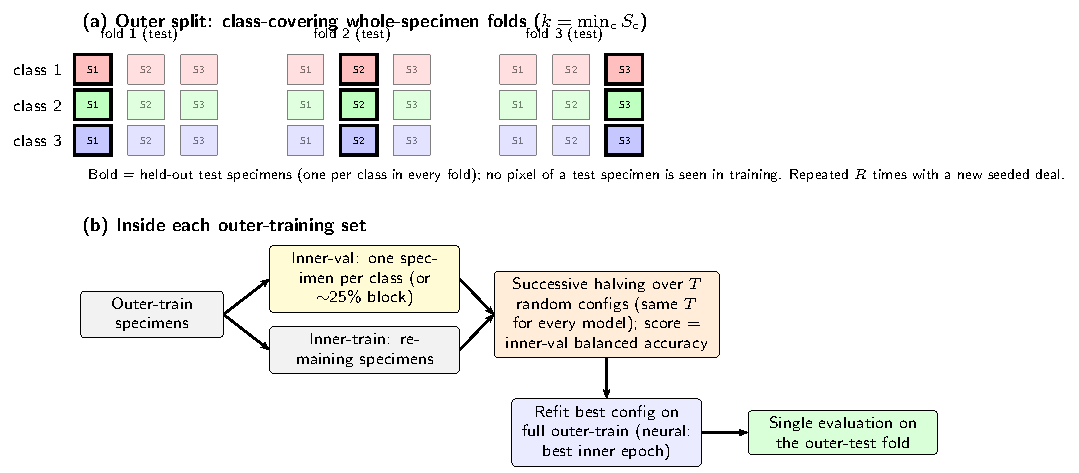
\includegraphics[width=0.85\textwidth]{figures/fig_protocol.pdf}
\caption{Evaluation protocol. (a) Outer folds hold out whole specimens and always contain at least one specimen of every class. (b) Inside each outer-training set, one specimen per class is held out for model selection; successive halving selects a configuration with the same budget $T$ for every model, which is refit on all training specimens and evaluated once on the test fold.}
\label{fig:protocol}
\end{figure*}

Model definitions, search spaces and preprocessing options were frozen before the final benchmark sweep. Collagen Acetic Acid was used for architecture exploration with its own cross-validation. Outer-test folds were not used to tune individual model configurations. The number of spectral repeats was later increased after the first two repeats had been inspected; this post-hoc change is described below and applied equally to all spectral models.

\subsection{Motivation: what the prototype got wrong}\label{sec:motivation}
The first audit concerns the earlier prototype. It aligned emission bands by index, which placed 31 real wavelengths onto 30 positions on the development set. Its specimen split also failed to guarantee class coverage: with seed 42, two of the three test folds had class sets $[1,1,2]$ and $[0,0,2]$. After wavelength alignment and class-covering folds, whole-specimen balanced accuracy for the same prototype family changed from 79.8--81.5\% to 81.7--82.7\% across three historical edge-handling modes, while logistic regression changed from 63.7\% to 73.8\%. The three prototype edge modes were circular wrapping, zero padding, and discarding edge-centred tokens; circular wrapping was later removed from the frozen search space. These are early fixed-configuration audit results. A separate comparison used default configurations to contrast random-pixel and whole-specimen evaluation. Random-pixel splits gave 97.9\% for logistic regression, 98.4\% for the MLP and 98.4\% for the prototype. Whole-specimen folds gave 87.8\%, 86.8\% and 88.3\%, respectively, a gap of 10--12 points. A third sensitivity check used five different specimen fold assignments with fixed configurations and gave 81.1$\pm$0.8\% for attention and 76.2$\pm$2.1\% for logistic regression. These three groups of numbers come from different development experiments and are not directly comparable as one model ranking.

\subsection{Outer folds}
Let $S_c$ be the number of specimens of class $c$ and $k=\min_c S_c$. For repeat $r=0,\dots,R-1$ the specimens of each class are shuffled with seed $r$ and dealt round-robin into $k$ folds, so every fold contains at least one specimen of every class; this is asserted in code. Repeats were limited by compute (see Sec.~\ref{sec:limits}). The sweep started with $R=2$ for Pepsin ($k=3$, 6 units), $R=2$ for Lichens~2 ($k=2$, 4 units) and $R=1$ for Lichens~1 ($k=4$, 4 units). After seeing the first two repeats of the spectral track we extended the spectral models to $R=5$ on Pepsin (15 units) and Lichens~2 (10 units) to gain statistical power; the extension was applied equally to all 12 spectral models, and Lichens~1 was not extended (accuracies near ceiling, highest cost). Spatial-track models keep the initial 6, 4 and 4 units. All comparisons are between models run on identical outer folds. Test pixels of one fold belong to specimens that do not appear in the training set.

\subsection{Inner validation and tuning}
Within each outer-training set, one specimen per class is held out as inner-validation (chosen at random with a seed); if a class has a single training specimen, a spatially contiguous 25\% block along the longer axis of that specimen is held out instead. Every model is tuned by random search over its own search space with the same configuration-count budget, $T=3$ configurations (the default configuration is candidate~0 and two are drawn at random). For neural models, selection uses successive halving~\cite{jamieson2016successive,li2018hyperband}: all $T$ candidates are trained for $\lceil E_{\max}/5\rceil$ epochs, the better half is trained for $\lceil E_{\max}/2\rceil$ epochs and the better half of those for $E_{\max}=25$ epochs (5, 13 and 25 epochs; early stopping with patience 6 on inner-validation balanced accuracy). The planned larger budget ($T=8$, $E_{\max}=40$, more repeats) was reduced because of compute constraints (Sec.~\ref{sec:limits}). Classical models are fit for each of the $T$ configurations. The score is inner-validation balanced accuracy. The best configuration is refit on all training specimens (neural models: for the best inner epoch, at least three) and evaluated once on the test fold. Random search is used for its efficiency over grids~\cite{bergstra2012random}; nesting avoids selection bias in the reported estimate~\cite{cawley2010overfitting}. This matches the number of candidate configurations, not wall-clock compute, across model families~\cite{gulrajani2021domainbed}.

\subsection{Shared preprocessing and training}\label{sec:preproc}
Preprocessing is part of every model's search space, with the same options for all: per-pixel normalisation $\in\{$none, $L_2$, area$\}$ applied across all features (global scope; per-excitation scope was dropped after the development experiments), an optional $\log(1+x/s)$ transform ($s$ the median positive training value), and per-feature standardisation. Statistics are fitted on training pixels only. All neural models, baselines and ours, share one training loop: AdamW~\cite{loshchilov2019adamw} with linear warm-up (3 epochs) and cosine decay, weight decay $10^{-4}$, gradient-norm clipping, label smoothing 0.05, and specimen-balanced sampling with replacement (500 pixels per specimen and epoch), which gives each training specimen the same expected weight regardless of its pixel count. Shared options are the same for all neural models: augmentation $\in\{$none, scaling plus noise$\}$ (log-uniform scale in $[0.7,1.4]$, an exact no-op whenever normalisation is on, plus Gaussian noise of 1\% of the feature standard deviation), excitation dropout $\in\{0,0.25\}$ (whole excitation blocks zeroed after preprocessing), and learning rate $\in\{3\!\times\!10^{-4},10^{-3},3\!\times\!10^{-3}\}$. Early stopping monitors inner-validation balanced accuracy. Classical models use the same preprocessing and specimen-balanced sample weights (or specimen-balanced subsampling where the method has no weights).

\subsection{Baselines}
\emph{Spectral track (8):} logistic regression, RBF SVM, random forest, histogram gradient boosting, $k$-NN, MLP, 1D-CNN over the (excitation, emission)-sorted feature vector, and pixel-wise SpectralFormer~\cite{hong2022spectralformer}. \emph{Spatial track (5):} logistic regression and random forest on the concatenation of the centre spectrum and the patch-mean spectrum, 2D-CNN~\cite{chen2016cnnhsi,hamida20183d}, patch-wise SpectralFormer~\cite{hong2022spectralformer}, and SSFTT~\cite{sun2022ssftt}. Deep spatial baselines are scaled down to the 150--210 features and 5--7 pixel patches of our data. Patch size is $P\in\{5,7\}$; to bound cost, training and inner-validation pixels are capped at 2000 per specimen (a fixed random subset), while test folds are evaluated on all pixels. Linear SVM, extra trees, a band-token vision transformer, a 3D-CNN and HybridSN~\cite{roy2020hybridsn} were implemented but dropped from the final sweep for cost and redundancy with the retained models. Pre-trained foundation models such as SpectralGPT~\cite{hong2024spectralgpt} were not run because their input assumptions (fixed band layout, remote-sensing pre-training) do not match ME fluorescence data.

\subsection{Metrics}
The primary metric is pixel-level balanced accuracy (mean per-class recall) on the pooled test pixels of a fold. We also report macro-F1, pixel accuracy, specimen-averaged accuracy (mean over test specimens of their pixel accuracy), specimen majority-vote accuracy, per-class recall and the confusion matrix. Labels are fixed to $0,\dots,C-1$ so that metrics are comparable across folds.

\subsection{Statistics}
The unit of analysis is a (repeat, fold) pair. We report paired mean differences in balanced accuracy, Wilcoxon signed-rank tests, the Nadeau--Bengio corrected resampled $t$-test~\cite{nadeau2003inference}, and bootstrap 95\% intervals of the paired mean difference. The corrected statistic is $t=\bar d/\sqrt{(1/n+n_{\mathrm{te}}/n_{\mathrm{tr}})s_d^2}$ and accounts for overlap between training sets. The bootstrap resamples repeat/fold units and is therefore descriptive because those units are correlated. Table~\ref{tab:stats} reports unadjusted corrected-test $p$-values and Holm-adjusted Wilcoxon $p$-values~\cite{holm1979simple}. We use the corrected test as the inferential reference and do not treat isolated unadjusted $p<0.05$ values as multiplicity-controlled evidence. Datasets are reported separately and are not pooled. We do not use a Nemenyi or critical-difference analysis because there are only three processed datasets and the two lichen datasets are not independent biological cohorts.

\section{Results}\label{sec:results}
All results are from the final evaluation sweep: $T=\BudgetT$ configurations per model, $E_{\max}=\MaxEpochsE$ epochs, $R=5$ repeats on Pepsin and Lichens~2 and $R=1$ on Lichens~1 for the spectral models (15, 10 and 4 units), and 6, 4 and 4 units for the spatial models, on one Apple M4 Pro GPU (MPS) shared with other jobs. All (repeat, fold, model) jobs completed. The four Lichens~1 spatial-attention jobs first failed with an out-of-memory error and were rerun later with the same settings; the rerun results are used. Where tables refer to the ``best'' proposed variant, this means the variant with the highest mean balanced accuracy on the outer-test units of that dataset. This is a post-hoc descriptive choice and is optimistically biased. We therefore do not use those rows to claim generalisable superiority.

\subsection{Spectral track}
\begin{table*}[!t]
\centering
\caption{Spectral track: balanced accuracy (\%), mean $\pm$ std over (repeat, fold) units. Best per column in bold, second best underlined. Models below the rule are our attention family (ex tokens v2: excitation tokens; ME-Attn (meas.): measurement tokens; SmartAttn v0: reference prototype). The $\Delta$ row compares the highest-mean proposed variant with the highest-mean baseline on the same outer-test units. Both are identified post hoc, so this row is descriptive.}
\label{tab:spectral}
\small
\begin{tabular}{lccc}
\toprule
Model & Collagen Pepsin & Lichens 1 & Lichens 2 \\
\midrule
LR & \underline{90.3 $\pm$ 9.2} & 99.2 $\pm$ 0.3 & 83.3 $\pm$ 7.8 \\
RBF-SVM & 87.3 $\pm$ 8.1 & \underline{99.3 $\pm$ 0.4} & \textbf{86.6 $\pm$ 7.0} \\
RF & 83.7 $\pm$ 9.0 & 98.6 $\pm$ 0.8 & 83.2 $\pm$ 7.4 \\
HGB & 84.7 $\pm$ 6.9 & 97.5 $\pm$ 3.5 & 84.6 $\pm$ 7.5 \\
kNN & 81.3 $\pm$ 8.9 & 91.8 $\pm$ 5.7 & 83.5 $\pm$ 7.0 \\
MLP & 83.2 $\pm$ 13.0 & 98.8 $\pm$ 0.6 & 85.6 $\pm$ 5.6 \\
1D-CNN & 79.2 $\pm$ 9.3 & 98.0 $\pm$ 1.1 & 81.6 $\pm$ 5.8 \\
SpectralFormer & 83.9 $\pm$ 10.3 & \textbf{99.5 $\pm$ 0.1} & 86.1 $\pm$ 6.3 \\
\midrule
SmartAttn v0 & 80.5 $\pm$ 12.6 & 98.8 $\pm$ 0.8 & 83.4 $\pm$ 6.9 \\
ME-Attn (meas.) & 85.2 $\pm$ 9.2 & 98.2 $\pm$ 1.3 & 83.1 $\pm$ 5.2 \\
ex tokens v2 & \textbf{91.1 $\pm$ 7.6} & 98.8 $\pm$ 0.8 & \underline{86.5 $\pm$ 5.8} \\
hybrid conv attn & 79.7 $\pm$ 11.2 & 95.5 $\pm$ 4.6 & 82.3 $\pm$ 7.1 \\
\midrule
Best ours $-$ best baseline [95\% CI] & $+0.8$ [$-1.5$, $+3.1$] & $-0.6$ [$-1.3$, $-0.1$] & $-0.1$ [$-1.0$, $+0.8$] \\
Strongest baseline & LR & SpectralFormer & RBF-SVM \\
\midrule
Units $n$ & 15 & 4 & 10 \\
\bottomrule
\end{tabular}

\end{table*}

Table~\ref{tab:spectral} gives the spectral-track results. The excitation-token model (\texttt{ex\_tokens\_v2}) has the highest mean among all models on Collagen Pepsin (\BestOursAccPepsinSpectral\,$\pm$\,\BestOursStdPepsinSpectral\%). On Lichens~2 its mean is \BestOursAccLichensTwoSpectral\%, 0.1 points below the RBF SVM. On Lichens~1 its mean is \BestOursAccLichensOneSpectral\%, 0.6 points below SpectralFormer, with only four repeat/fold units. Relative to the highest-mean baseline in each dataset, the paired differences are \GapPepsinSpectral{} [\GapLoPepsinSpectral, \GapHiPepsinSpectral] points on Pepsin, \GapLichensOneSpectral{} [\GapLoLichensOneSpectral, \GapHiLichensOneSpectral] on Lichens~1, and \GapLichensTwoSpectral{} [\GapLoLichensTwoSpectral, \GapHiLichensTwoSpectral] on Lichens~2. These comparisons do not establish that the excitation-token model is superior to the strongest tuned baseline on any dataset.

Table~\ref{tab:stats} gives the paired statistics. Several Pepsin and Lichens~2 comparisons have small Holm-adjusted Wilcoxon $p$-values. The Wilcoxon calculation treats repeat/fold units as independent even though they reuse the same specimens, so we do not use those results to claim generalisable superiority. Under the Nadeau--Bengio corrected $t$-test, the unadjusted $p$-values fall below 0.05 only for $k$-NN on Pepsin ($p_{\mathrm{NB}}=0.024$) and the 1D-CNN on Lichens~2 ($p_{\mathrm{NB}}=0.029$). These corrected-test $p$-values are not multiplicity adjusted. Taken together, the tests support the narrower conclusion that the excitation-token model is competitive with the strongest baselines, not that it is reliably superior.

\begin{table*}[!t]
\centering
\caption{Paired comparison of our attention variants and baselines, one block per dataset and track. First rows of each block: every attention variant against the strongest baseline (Holm across variants). Remaining rows: our best variant (marked $^*$, selected on the test units, hence optimistic) against every other baseline (Holm across baselines). $n$: units; $\bar d$: mean difference in balanced accuracy in points with bootstrap 95\% CI; W/T/L: wins, ties, losses; $p_{\mathrm{W}}$: Wilcoxon $p$ (unadjusted), $p_{\mathrm{NB}}$: Nadeau--Bengio corrected $t$-test $p$ (unadjusted), $p_{\mathrm{W}}^{\mathrm{Holm}}$: Holm-adjusted Wilcoxon $p$. With $n=4$ the smallest attainable two-sided Wilcoxon $p$ is 0.125.}
\label{tab:stats}
\scriptsize
\setlength{\tabcolsep}{3pt}
% * = best 'ours' variant by mean balanced accuracy (selected on test units: optimistic).
% Rows vs the strongest baseline list every 'ours' variant; Holm across the 'ours' variants.
% Remaining rows: best ours vs every other baseline; Holm across baselines.
% p_NB: Nadeau-Bengio corrected resampled t-test with mean n_test/n_train.
\small
\begin{tabular}{llllcclccc}
\toprule
Track & Dataset & Ours & vs. & n & $\bar d$ [95\% CI] & W/T/L & $p_{\mathrm{W}}$ & $p_{\mathrm{NB}}$ & $p_{\mathrm{W}}^{\mathrm{Holm}}$ \\
\midrule
spectral & Collagen Pepsin & SmartAttn v0 & LR & 15 & $-9.9$ [$-14.3$, $-5.5$] & 2/0/13 & 0.001 & 0.172 & 0.005 \\
spectral & Collagen Pepsin & ME-Attn (meas.) & LR & 15 & $-5.2$ [$-10.5$, $+0.1$] & 4/0/11 & 0.095 & 0.536 & 0.189 \\
spectral & Collagen Pepsin & ex tokens v2* & LR & 15 & $+0.8$ [$-1.5$, $+3.1$] & 9/0/6 & 0.454 & 0.823 & 0.454 \\
spectral & Collagen Pepsin & hybrid conv attn & LR & 15 & $-10.6$ [$-16.2$, $-5.6$] & 4/0/11 & 0.003 & 0.221 & 0.010 \\
spectral & Collagen Pepsin & ex tokens v2* & RBF-SVM & 15 & $+3.8$ [$+1.2$, $+6.4$] & 12/0/3 & 0.010 & 0.359 & 0.031 \\
spectral & Collagen Pepsin & ex tokens v2* & RF & 15 & $+7.5$ [$+3.9$, $+11.0$] & 13/0/2 & 0.003 & 0.193 & 0.016 \\
spectral & Collagen Pepsin & ex tokens v2* & HGB & 15 & $+6.5$ [$+3.1$, $+9.6$] & 12/0/3 & 0.004 & 0.211 & 0.021 \\
spectral & Collagen Pepsin & ex tokens v2* & kNN & 15 & $+9.8$ [$+7.6$, $+12.6$] & 15/0/0 & <0.001 & 0.024 & <0.001 \\
spectral & Collagen Pepsin & ex tokens v2* & MLP & 15 & $+7.9$ [$+2.3$, $+14.1$] & 11/0/4 & 0.026 & 0.398 & 0.051 \\
spectral & Collagen Pepsin & ex tokens v2* & 1D-CNN & 15 & $+11.9$ [$+7.5$, $+16.6$] & 14/0/1 & <0.001 & 0.113 & 0.002 \\
spectral & Collagen Pepsin & ex tokens v2* & SpectralFormer & 15 & $+7.2$ [$+3.1$, $+11.6$] & 11/0/4 & 0.005 & 0.293 & 0.021 \\
\midrule
spectral & Lichens 1 & SmartAttn v0 & SpectralFormer & 4 & $-0.7$ [$-1.3$, $-0.0$] & 1/0/3 & 0.250 & 0.329 & 0.750 \\
spectral & Lichens 1 & ME-Attn (meas.) & SpectralFormer & 4 & $-1.3$ [$-2.2$, $-0.4$] & 1/0/3 & 0.250 & 0.237 & 0.750 \\
spectral & Lichens 1 & ex tokens v2* & SpectralFormer & 4 & $-0.6$ [$-1.3$, $-0.1$] & 1/0/3 & 0.250 & 0.306 & 0.750 \\
spectral & Lichens 1 & hybrid conv attn & SpectralFormer & 4 & $-4.0$ [$-8.6$, $-1.1$] & 0/0/4 & 0.125 & 0.326 & 0.500 \\
spectral & Lichens 1 & ex tokens v2* & LR & 4 & $-0.3$ [$-1.0$, $+0.3$] & 1/0/3 & 0.375 & 0.619 & 1.000 \\
spectral & Lichens 1 & ex tokens v2* & RBF-SVM & 4 & $-0.5$ [$-0.8$, $-0.1$] & 1/0/3 & 0.250 & 0.254 & 1.000 \\
spectral & Lichens 1 & ex tokens v2* & RF & 4 & $+0.2$ [$-0.2$, $+0.7$] & 3/0/1 & 0.625 & 0.633 & 1.000 \\
spectral & Lichens 1 & ex tokens v2* & HGB & 4 & $+1.3$ [$-0.7$, $+4.8$] & 1/0/3 & 0.875 & 0.646 & 1.000 \\
spectral & Lichens 1 & ex tokens v2* & kNN & 4 & $+7.0$ [$+2.9$, $+12.7$] & 4/0/0 & 0.125 & 0.216 & 1.000 \\
spectral & Lichens 1 & ex tokens v2* & MLP & 4 & $-0.0$ [$-0.5$, $+0.5$] & 2/0/2 & 1.000 & 0.992 & 1.000 \\
spectral & Lichens 1 & ex tokens v2* & 1D-CNN & 4 & $+0.8$ [$+0.5$, $+1.1$] & 4/0/0 & 0.125 & 0.064 & 1.000 \\
\midrule
spectral & Lichens 2 & SmartAttn v0 & RBF-SVM & 10 & $-3.2$ [$-5.6$, $-1.0$] & 3/0/7 & 0.027 & 0.458 & 0.059 \\
spectral & Lichens 2 & ME-Attn (meas.) & RBF-SVM & 10 & $-3.5$ [$-5.3$, $-1.7$] & 2/0/8 & 0.014 & 0.313 & 0.055 \\
spectral & Lichens 2 & ex tokens v2* & RBF-SVM & 10 & $-0.1$ [$-1.0$, $+0.8$] & 6/0/4 & 1.000 & 0.950 & 1.000 \\
spectral & Lichens 2 & hybrid conv attn & RBF-SVM & 10 & $-4.2$ [$-10.0$, $-0.7$] & 2/0/8 & 0.020 & 0.657 & 0.059 \\
spectral & Lichens 2 & ex tokens v2* & LR & 10 & $+3.1$ [$+1.3$, $+4.9$] & 9/0/1 & 0.014 & 0.361 & 0.082 \\
spectral & Lichens 2 & ex tokens v2* & RF & 10 & $+3.2$ [$+1.7$, $+4.6$] & 9/0/1 & 0.006 & 0.238 & 0.041 \\
spectral & Lichens 2 & ex tokens v2* & HGB & 10 & $+1.9$ [$+0.6$, $+3.1$] & 8/0/2 & 0.020 & 0.432 & 0.098 \\
spectral & Lichens 2 & ex tokens v2* & kNN & 10 & $+2.9$ [$+1.2$, $+4.7$] & 7/0/3 & 0.027 & 0.374 & 0.109 \\
spectral & Lichens 2 & ex tokens v2* & MLP & 10 & $+0.9$ [$-0.1$, $+2.0$] & 6/0/4 & 0.275 & 0.656 & 0.826 \\
spectral & Lichens 2 & ex tokens v2* & 1D-CNN & 10 & $+4.9$ [$+3.8$, $+5.9$] & 10/0/0 & 0.002 & 0.029 & 0.016 \\
spectral & Lichens 2 & ex tokens v2* & SpectralFormer & 10 & $+0.4$ [$-0.3$, $+1.2$] & 6/0/4 & 0.375 & 0.776 & 0.826 \\
\midrule
spatial & Collagen Pepsin & ME-Attn (spatial)* & Patch-mean RF & 6 & $+1.4$ [$-6.1$, $+7.7$] & 4/0/2 & 0.688 & 0.862 & 0.688 \\
spatial & Collagen Pepsin & ME-Attn (spatial)* & Patch-mean LR & 6 & $+6.0$ [$-0.6$, $+13.1$] & 3/0/3 & 0.438 & 0.483 & 1.000 \\
spatial & Collagen Pepsin & ME-Attn (spatial)* & 2D-CNN & 6 & $+4.9$ [$-3.7$, $+14.5$] & 3/0/3 & 0.688 & 0.656 & 1.000 \\
spatial & Collagen Pepsin & ME-Attn (spatial)* & SpectralFormer-P & 6 & $+3.5$ [$-6.7$, $+14.5$] & 5/0/1 & 0.312 & 0.767 & 1.000 \\
spatial & Collagen Pepsin & ME-Attn (spatial)* & SSFTT & 6 & $+2.8$ [$-7.4$, $+13.7$] & 2/0/4 & 1.000 & 0.821 & 1.000 \\
\midrule
spatial & Lichens 1 & ME-Attn (spatial)* & 2D-CNN & 4 & $-0.6$ [$-1.0$, $-0.1$] & 0/0/4 & 0.125 & 0.254 & 0.125 \\
spatial & Lichens 1 & ME-Attn (spatial)* & Patch-mean LR & 4 & $-0.3$ [$-0.8$, $+0.2$] & 2/0/2 & 0.625 & 0.581 & 1.000 \\
spatial & Lichens 1 & ME-Attn (spatial)* & Patch-mean RF & 4 & $-0.3$ [$-0.9$, $+0.4$] & 2/0/2 & 0.625 & 0.695 & 1.000 \\
spatial & Lichens 1 & ME-Attn (spatial)* & SpectralFormer-P & 4 & $+0.3$ [$-0.4$, $+1.0$] & 3/0/1 & 0.625 & 0.667 & 1.000 \\
spatial & Lichens 1 & ME-Attn (spatial)* & SSFTT & 4 & $-0.5$ [$-1.4$, $-0.0$] & 1/0/3 & 0.250 & 0.504 & 1.000 \\
\midrule
spatial & Lichens 2 & ME-Attn (spatial)* & 2D-CNN & 4 & $-1.5$ [$-3.6$, $-0.1$] & 0/0/4 & 0.125 & 0.577 & 0.125 \\
spatial & Lichens 2 & ME-Attn (spatial)* & Patch-mean LR & 4 & $+1.6$ [$+0.3$, $+3.6$] & 4/0/0 & 0.125 & 0.548 & 0.625 \\
spatial & Lichens 2 & ME-Attn (spatial)* & Patch-mean RF & 4 & $+1.8$ [$-0.2$, $+4.3$] & 3/0/1 & 0.250 & 0.593 & 0.625 \\
spatial & Lichens 2 & ME-Attn (spatial)* & SpectralFormer-P & 4 & $+0.6$ [$-1.7$, $+2.5$] & 3/0/1 & 0.875 & 0.845 & 0.875 \\
spatial & Lichens 2 & ME-Attn (spatial)* & SSFTT & 4 & $-0.5$ [$-0.8$, $-0.1$] & 0/0/4 & 0.125 & 0.396 & 0.625 \\
\bottomrule
\end{tabular}

\end{table*}

The other attention variants are below the best baselines (Table~\ref{tab:spectral}). Measurement tokens, the reference prototype and the convolutional-stem hybrid are 5.2, 9.9 and 10.6 points below logistic regression on Pepsin, and 3.5, 3.2 and 4.2 points below the RBF SVM on Lichens~2; on Pepsin the differences to logistic regression of the prototype and the hybrid are significant by the Holm-adjusted Wilcoxon test (0.005 and 0.010) but not by the corrected $t$-test ($p_{\mathrm{NB}}>0.17$). Within our family, tokenising whole emission spectra per excitation gives higher observed means than tokenising single measurements in this data regime. Because the family differs in several aspects at once (tokenisation, sequence length, embedding, search space), this is a comparison of members, not an isolating ablation.

\subsection{Spatial track}
\begin{table*}[!t]
\centering
\caption{Oracle-masked spatial track: balanced accuracy (\%), mean $\pm$ std over units (6, 4 and 4). Patch size $P$ is tuned in $\{5,7\}$. All spatial models use annotation-derived component boundaries when constructing patches. Best per column is bold and second best is underlined. The $\Delta$ row is descriptive and compares the highest-mean proposed spatial model with the highest-mean baseline.}
\label{tab:spatial}
\small
\begin{tabular}{lccc}
\toprule
Model & Collagen Pepsin & Lichens 1 & Lichens 2 \\
\midrule
Patch-mean LR & 81.9 $\pm$ 15.4 & 99.4 $\pm$ 0.5 & 84.0 $\pm$ 3.9 \\
Patch-mean RF & \underline{86.4 $\pm$ 10.0} & 99.3 $\pm$ 0.5 & 83.8 $\pm$ 4.5 \\
2D-CNN & 82.9 $\pm$ 13.1 & \textbf{99.6 $\pm$ 0.2} & \textbf{87.1 $\pm$ 3.4} \\
SpectralFormer-P & 84.3 $\pm$ 17.6 & 98.7 $\pm$ 1.3 & 84.9 $\pm$ 3.5 \\
SSFTT & 85.1 $\pm$ 14.8 & \underline{99.6 $\pm$ 0.6} & \underline{86.0 $\pm$ 1.6} \\
\midrule
ME-Attn (spatial) & \textbf{87.9 $\pm$ 14.3} & 99.1 $\pm$ 0.8 & 85.6 $\pm$ 1.9 \\
\midrule
Best ours $-$ best baseline [95\% CI] & $+1.4$ [$-6.1$, $+7.7$] & $-0.6$ [$-1.0$, $-0.1$] & $-1.5$ [$-3.6$, $-0.1$] \\
Strongest baseline & Patch-mean RF & 2D-CNN & 2D-CNN \\
\midrule
Units $n$ & 6 & 4 & 4 \\
\bottomrule
\end{tabular}

\end{table*}

Table~\ref{tab:spatial} reports the oracle-masked spatial track, with the same paired statistics in Table~\ref{tab:stats}. Spatial attention has the highest mean on Pepsin (\BestOursAccPepsinSpatial\,$\pm$\,\BestOursStdPepsinSpatial\%) but the difference to the patch-mean random forest, \GapPepsinSpatial{} [\GapLoPepsinSpatial, \GapHiPepsinSpatial] points over six units, is far inside the fold-to-fold spread (standard deviations of 10 to 18 points for all spatial models on Pepsin). It is below the strongest baseline on Lichens~1 (\BestOursAccLichensOneSpatial\% against \BestBaseAccLichensOneSpatial\% for the 2D-CNN) and Lichens~2 (\BestOursAccLichensTwoSpatial\% against \BestBaseAccLichensTwoSpatial\%, \GapLichensTwoSpatial{} [\GapLoLichensTwoSpatial, \GapHiLichensTwoSpatial] points, four losses in four units; Holm-adjusted Wilcoxon $p=\PHolmLichensTwoSpatial$, the smallest value attainable with four units). The 2D-CNN is the strongest spatial baseline on Lichens~1 and Lichens~2. Spatial context does not improve over the best spectral-only model on Pepsin (best spatial mean \BestOursAccPepsinSpatial\% on six units against \BestOursAccPepsinSpectral\% for \texttt{ex\_tokens\_v2} on 15; the unit sets differ, so this is indicative only), and on Lichens~1 and Lichens~2 the best spatial and best spectral means differ by less than 1 point (99.6 vs 99.5 and 87.1 vs 86.6). Under this oracle-boundary setting, we find no reliable benefit of spatial context or spatial attention. Because the boundary mask comes from the annotation, this result should not be interpreted as deployment performance.

\subsection{Per-dataset comparison}
\begin{figure*}[!t]
\centering
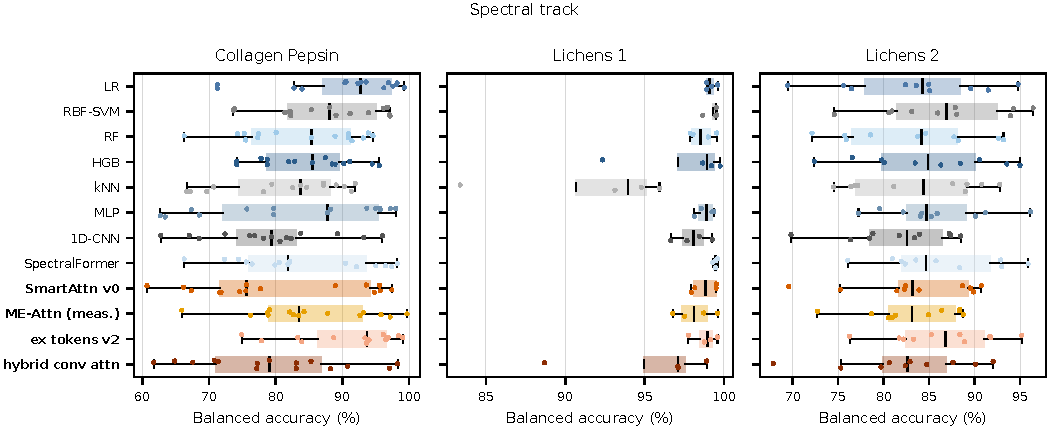
\includegraphics[width=\textwidth]{generated/figures/fig_box_spectral.pdf}
\caption{Spectral track: distribution of balanced accuracy over (repeat, fold) units for every model, one panel per dataset (box: quartiles and median; points: units). Attention variants are in the lower four rows.}
\label{fig:box}
\end{figure*}
Fig.~\ref{fig:box} shows the distribution of the spectral-track results. Variation across units dominates variation across models: on Pepsin the standard deviation over units is 7 to 13 points for all models, and the interquartile ranges of the top models overlap almost completely, so the ranking depends on which specimens are in the test folds (specimen heterogeneity). On Lichens~1 the standard deviations are below 1.5 points for all models except the $k$-NN, the hybrid and gradient boosting, and every strong model is above 98\%; on Lichens~2 they are 5 to 8 points. Pixel-level metrics understate specimen-level performance: the specimen majority-vote accuracy of \texttt{ex\_tokens\_v2} is 95.6\% on Pepsin (93.3\% for logistic regression, the RBF SVM and gradient boosting) and 100\% on Lichens~1 for every model, and 92.3\% on Lichens~2 (best: $k$-NN, 96.5\%), with large standard deviations given so few specimens. The class with only two regions in Lichens~2 contributes at most two test specimens per repeat, so its recall is estimated from very few independent regions.

\subsection{Attention and feature importance versus wavelength selection}\label{sec:importance}
\begin{figure*}[!t]
\centering
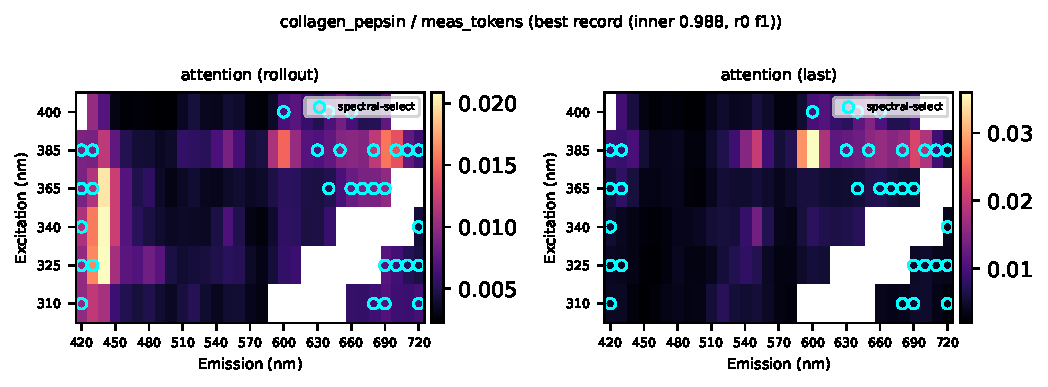
\includegraphics[width=\textwidth]{generated/importance/collagen_pepsin_meas_tokens/collagen_pepsin_meas_tokens/importance_heatmap.pdf}\\[4pt]
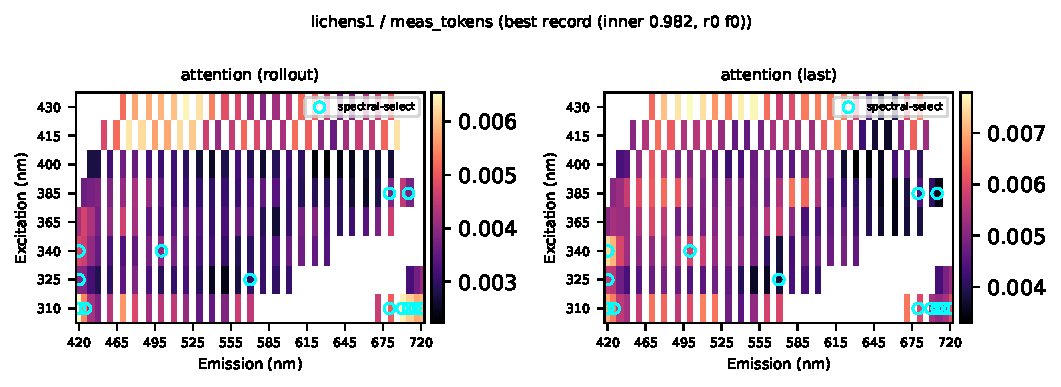
\includegraphics[width=\textwidth]{generated/importance/lichens1_meas_tokens/lichens1_meas_tokens/importance_heatmap.pdf}
\caption{Measurement-token importance on the (excitation, emission) grid for one retrained outer-test fold per dataset (repeat 0, fold 0; top: Collagen Pepsin, bottom: Lichens~1). Each row shows attention rollout and last-layer attention. Circles mark measurements chosen by the unsupervised selection method~\cite{meloyan2026unsupervised}. White cells are absent measurements.}
\label{fig:importance}
\end{figure*}
We compare attention-derived importance with the wavelengths selected by the unsupervised convolutional-autoencoder method of~\cite{meloyan2026unsupervised} (30 selected measurements for Pepsin and 13 for Lichens~1; no selection is available for Lichens~2). For each dataset and model we take the configuration of the sweep record with the highest inner-validation score, retrain it once on the outer-training specimens of repeat~0, fold~0 (with the same inner split for early stopping), and compute attention rollout and last-layer attention averaged over up to 4000 pixels of the held-out test fold. Because this uses a single fold per dataset, the results below are descriptive and should be read as such; importance scores are not causal~\cite{jain2019notexpl}.

For the measurement-token model, the 30 measurements with the highest rollout importance on Pepsin include 13 of the 30 selected by the unsupervised method, against 5.7 expected by chance (hypergeometric $p=0.0005$; Spearman correlation between importance and selection indicator $\rho=0.48$). On Lichens~1 the overlap is 4 of 13 against 0.9 expected ($p=0.007$, $\rho=0.13$). On Pepsin the rollout concentrates on the 440\,nm emission band under the 325, 340 and 365\,nm excitations and the selected measurements lie at the short-wavelength end of the emission range and in the long-wavelength tails (Fig.~\ref{fig:importance}). The excitation-token model, by construction, assigns importance to whole excitations: its attention concentrates on the 415\,nm excitation in both lichen datasets and on 325\,nm (rollout) and 385\,nm (last layer) in Pepsin. A band-level overlap with the selected measurements is not meaningful for it, since all emission bands of one excitation share one score, and we do not interpret the overlap values computed for it. The set overlap is above chance in these two single-fold analyses. The two signals are not both label-free: the attention scores come from a supervised classifier, whereas the comparison selector is unsupervised. The Lichens~1 rank correlation is weak ($\rho=0.13$). These results do not show that either method identifies measurements that are causally important for classification, and we did not retrain classifiers on the top-ranked measurements.

\section{Discussion}
Under whole-specimen evaluation with matched configuration counts, the observed advantage of attention over strong tuned baselines is small or absent. The excitation-token model has the strongest means within the proposed family and the highest overall mean on Pepsin, but the corrected tests do not establish superiority over the strongest baseline on any dataset. On Lichens~1 its mean is 0.6 points below SpectralFormer, and on Lichens~2 it is 0.1 points below the RBF SVM. The remaining attention variants have lower means on Pepsin and Lichens~2.

\emph{Why excitation tokens and not measurement tokens.} We can state what the data show and offer hypotheses that we did not test. Every attention variant has the same training data: a few specimens per class, so the number of independent examples is very small compared with the number of pixels, and inter-specimen variance dominates (Fig.~\ref{fig:box}). Measurement tokens present 150--210 tokens that the model must aggregate with a small search and training budget. The default excitation-token configuration instead presents 6--8 tokens, each representing one excitation spectrum. This representation exposes cross-excitation relations with a much shorter sequence and imposes a stronger structural constraint. This is consistent with the development finding that per-excitation normalisation lowers accuracy by 4--8 points because the cross-excitation intensity ratios are class-informative (Sec.~\ref{sec:dev}). The MLP, 1D-CNN and hybrid are also weaker than the linear model on Pepsin, which points to the amount of data and the tuning budget as limits for all flexible neural models, not to attention specifically. We did not run the wavelength-encoding ablations or the shuffled-wavelength control that would show whether the continuous wavelength encoding contributes anything beyond the intensity values; the results therefore do not support the claim that wavelength-aware encoding is the reason for the performance of the excitation-token model.

\emph{Statistical evidence.} The repeat/fold units are correlated (Sec.~\ref{sec:limits}). The corrected tests do not establish a reliable advantage over the strongest baseline on any dataset. Two individual corrected-test comparisons have unadjusted $p<0.05$, but those values are not multiplicity controlled. The small number of independent specimens or regions limits stronger inference.

\emph{Spatial context.} The oracle-masked spatial experiments do not show a reliable gain from adding a pixel neighbourhood (Table~\ref{tab:spatial}). We have not tested why. More importantly, the spatial track uses annotation-derived component boundaries at test time. It should therefore be treated as a controlled analysis of within-component context, not as evidence for a deployable spatial classifier.

\emph{Importance.} Measurement-token rankings overlap the unsupervised selected sets more than expected by chance on both analysed datasets. The Pepsin rank correlation is moderate, while the Lichens~1 correlation is weak. Since attention is obtained from a supervised classifier, this comparison does not represent agreement between two label-free signals and does not establish which measurements are most useful for classification.

\emph{Protocol versus model.} On the development set, random-pixel splits gave 97.9--98.4\% balanced accuracy and whole-specimen folds 86.8--88.3\% for the same models, a gap of 10--12 points (Sec.~\ref{sec:motivation}). This protocol effect is larger than the difference between our best attention model and the best baseline on every dataset (less than 1 point), and comparable to the spread between the best and the worst of the twelve spectral models on Pepsin (11.9 points); the protocol changes the measured accuracy more than the choice among the leading models does.

\section{Limitations}\label{sec:limits}
The number of independent biological specimens is small. Collagen Pepsin has three specimens per class and Lichens~1 has four. Lichens~2 has 2--10 annotated regions per class, but these regions are not equivalent to independent specimens and may share a thallus or imaging session. Lichens~1 and Lichens~2 also derive from the same underlying lichen material, so they are not independent biological replications. The spectral results contain 15, 4 and 10 correlated repeat/fold units, but those units reuse only 9, 16 and 28 specimen or region identifiers. Corrected tests therefore have low power; with four units no two-sided Wilcoxon $p$ below 0.125 is attainable.

The spatial track has an additional limitation. Patches are masked with annotation-derived specimen or region boundaries at test time. This supplies oracle boundary information and is not available in a general deployment setting unless an independent segmentation is provided. The spatial results should therefore be interpreted only within that oracle-boundary condition.

All data come from one instrument, so robustness to instrument change is not tested. Class labels come from region masks and may contain boundary errors. Search spaces are finite and the budget is small ($T=\BudgetT$ configurations, at most \MaxEpochsE{} epochs, 2--5 repeats). The planned larger budget was reduced because of compute constraints, and a larger search could change model rankings. The spectral repeat count was increased after the first two repeats had been inspected, although the extension was applied equally to all spectral models. Lichens~1 has only one repeat. The highest-mean proposed variant is also identified from the outer-test summaries, so comparisons labelled ``best ours'' are post hoc and optimistic.

The classical LR, SVM, tree and $k$-NN baselines use standard library implementations wrapped in the common evaluation harness. SpectralFormer and SSFTT are adapted implementations of published architectures, and the remaining neural baselines are implemented in the same project. No dedicated ablation isolates the wavelength encoding, Stokes-shift feature, relative bias or token dropout. We also did not run a shuffled-wavelength control or retrain classifiers using only the top-ranked importance measurements. The importance analysis uses a single outer-test fold per dataset. HybridSN, a 3D-CNN, linear SVM, extra trees, a band-token transformer and axial attention were implemented but were not included in the final sweep. Foundation models were not evaluated.

\section{Conclusion}
We evaluated attention-based ME-HSI classifiers with whole-specimen, class-covering splits, nested model selection and matched configuration counts. Excitation-level tokenisation gives the strongest observed means within the proposed family and the highest overall mean on Collagen Pepsin. It is within 0.1 points of the RBF SVM on Lichens~2 and below SpectralFormer on Lichens~1. The corrected tests do not establish that any attention variant is reliably better than the strongest tuned baseline. The oracle-masked spatial track also shows no reliable gain from spatial context. Measurement-token attention rankings have above-chance set overlap with an unsupervised selector, but this descriptive result does not establish causal feature importance. On the development set, changing from random-pixel to whole-specimen evaluation changes balanced accuracy by 10--12 points, more than the differences among the leading models. ME-HSI classification studies should therefore report specimen-level splits, matched model-selection budgets and statistical tests that account for repeated use of the same specimens.

\section*{Data and Code Availability}
Code, search spaces, the evaluation harness and result files are available at \RESULT{repository URL and commit}. The Lichens and Collagen data are on Zenodo~\cite{zenodo_lichens,zenodo_collagen}; \RESULT{confirm which datasets (Lichens~1, Lichens~2, Collagen Pepsin, Collagen Acetic) each record contains and whether Lichens~2 is released}. The unsupervised selection method used for comparison is described in~\cite{meloyan2026unsupervised}.

\bibliographystyle{IEEEtran}
\bibliography{refs}
\end{document}
